\documentclass[polish,11pt,a4paper]{article}
\usepackage[a4paper, margin=2cm]{geometry}
\usepackage[T1]{fontenc}
\usepackage{babel}
\usepackage{graphicx}
\usepackage{ragged2e}
\usepackage{caption}
\usepackage{amsmath} 
\usepackage{amssymb} 
\usepackage{setspace}
\usepackage[utf8]{inputenc}
\usepackage{subfig}
\usepackage{cancel}
\usepackage{import}
\usepackage{svg}
\usepackage{listings}
\usepackage[utf8]{inputenc}
\usepackage{booktabs}
\usepackage{lscape}
\usepackage{pdfpages}

\title{d}

\author{Dawid [Twoje Imię i Nazwisko]}
\date{\today}

\begin{document}
	
\lstset{ 
	language=Python, 
	basicstyle=\ttfamily, 
	keywordstyle=\color{blue}, 
	commentstyle=\color{green}, 
	stringstyle=\color{red}, 
	showstringspaces=false,
	numbers=left, 
	numberstyle=\tiny, 
	stepnumber=1, 
	numbersep=5pt, 
	backgroundcolor=\color{white}, 
	frame=single, 
	rulecolor=\color{black}, 
	tabsize=2, 
	captionpos=b, 
	breaklines=true, 
	breakatwhitespace=false
}	

%% Strona tytułowa
\setstretch{1.5}
\centering
\section*{POLITECHNIKA BIAŁOSTOCKA}

\section*{WYDZIAŁ MECHANICZNY}
\section*{PRACOWNIA SPECJALISTYCZNA}
\section*{ Sztuczne sieci neuronowe i systemy ekspertowe}
\section*{Ćwiczenie nr 3 }
\section*{Projektowanie optymalnego zespołu klasyfikatorów}
\large
KOD PRZEDMIOTU: MYAR2S22003M
\break
\large
\break
\break
\break

\raggedright
Autor: Ostaszewicz Dawid
\break

Kierunek: Automatyka i Robotyka, II stopień

Prowadzący: dr inż. Marcin Derlatka
\clearpage
\justifying	
\section*{Cel ćwiczenia}

Celem ćwiczenia jest zaprojektowanie i implementacja optymalnego zespołu klasyfikatorów dla przesłanego zbioru danych. Zespół ma obejmować co najmniej jeden klasyfikator realizujący każdą z technik: bagging, boosting oraz stacking. Zadanie obejmuje:

\begin{itemize}
	\item Wykorzystanie klasyfikatorów bazowych opartych na sieciach neuronowych, takich jak MLP (Multilayer Perceptron).
	\item Implementację klasyfikatorów bagging i boosting, takich jak BaggingClassifier, AdaBoostClassifier oraz GradientBoostingClassifier.
	\item Zastosowanie metody stacking, która łączy wyniki klasyfikatorów bazowych przy pomocy modelu meta-learnera, np. XGBoost.
	\item Eksperymentowanie z różnymi hiperparametrami klasyfikatorów oraz technikami optymalizacji, aby uzyskać jak najlepsze wyniki klasyfikacji.
\end{itemize}

\section{Wczytanie danych}
Dane wejściowe w formacie ARFF są wczytywane przy użyciu funkcji \texttt{arff.loadarff}. Zbiory danych są następnie konwertowane na format \texttt{pandas DataFrame} dla łatwiejszej manipulacji danymi.

\begin{lstlisting}[language=Python]
	Dry_Bean_Dataset_data, Dry_Bean_Dataset_meta = arff.loadarff('Dry_Bean_Dataset.arff')
	testing_beans_data, testing_beans_meta = arff.loadarff('testing_beans.arff')
	training_beans_data, training_beans_meta = arff.loadarff('training_beans.arff')
	
	Dry_Bean_Dataset = pd.DataFrame(Dry_Bean_Dataset_data)
	testing_beans = pd.DataFrame(testing_beans_data)
	training_beans = pd.DataFrame(training_beans_data)
\end{lstlisting}

\section{Przygotowanie danych}
W tej części skryptu wydzielamy cechy (\texttt{X}) i etykiety (\texttt{y}) zarówno z danych treningowych, jak i testowych. Etykiety są konwertowane z typu \texttt{byte} na \texttt{string}.

\begin{lstlisting}[language=Python]
	X_train = training_beans.drop('Class', axis=1)
	y_train = training_beans['Class']
	X_test = testing_beans.drop('Class', axis=1)  
	y_test = testing_beans['Class']

	y_train = y_train.str.decode('utf-8')  
	y_test = y_test.str.decode('utf-8')
\end{lstlisting}
\section{Kodowanie etykiet}
Użyto \texttt{LabelEncoder} do kodowania etykiet w postaci liczbowej, co jest wymagane do trenowania klasyfikatorów.

\begin{lstlisting}[language=Python]
	le = LabelEncoder()
	
	y_train = le.fit_transform(y_train)
	y_test = le.transform(y_test)
\end{lstlisting}

\section{Inicjalizacja klasyfikatorów}
Inicjalizowane są klasyfikatory bazowe: sieć neuronowa (\texttt{MLPClassifier}) oraz klasyfikator XGBoost (\texttt{XGBClassifier}). Sieć neuronowa jest używana w zespole bagging.

\begin{lstlisting}[language=Python]
	base_nn = MLPClassifier(hidden_layer_sizes=(100,), max_iter=500, random_state=42)
	xgb_clf = XGBClassifier(random_state=42)
\end{lstlisting}

\section{Bagging Classifier}
Tworzy się klasyfikator \texttt{BaggingClassifier}, który stosuje metodę bagging z wykorzystaniem sieci neuronowej jako klasyfikatora bazowego. Klasyfikator jest trenowany na danych treningowych, a następnie dokonujemy predykcji na danych testowych.

\begin{lstlisting}[language=Python]
	bagging_clf = BaggingClassifier(estimator=base_nn, n_estimators=10, random_state=42)
	bagging_clf.fit(X_train, y_train)
	y_pred_bagging = bagging_clf.predict(X_test)
\end{lstlisting}

\section{Boosting Classifier}
Następnie tworzymy klasyfikator boostingowy \texttt{GradientBoostingClassifier}, który jest trenowany na danych treningowych.

\begin{lstlisting}[language=Python]
	boosting_clf = GradientBoostingClassifier(n_estimators=50, random_state=42)
	boosting_clf.fit(X_train, y_train)
	y_pred_boosting = boosting_clf.predict(X_test)
\end{lstlisting}

\section{Stacking Classifier}
W przedstawionym fragmencie kodu zastosowano metodę stacking do łączenia predykcji trzech klasyfikatorów bazowych. Proces rozpoczyna się od zdefiniowania trzech modeli bazowych: bagging\_clf, boosting\_clf oraz xgb\_clf, które odpowiadają za generowanie predykcji na podstawie danych treningowych. Następnie, przy użyciu funkcji stacking, wykonywane jest połączenie wyników predykcji tych klasyfikatorów. Dla każdego modelu bazowego obliczane są predykcje "out-of-fold", które stanowią dane wejściowe do meta-learnera.

Funkcja stacking przyjmuje następujące parametry: dane treningowe X\_train, y\_train, dane testowe X\_test, oraz liczbę foldów kroswalidacji (n\_folds=4). Ustawienie regression=False wskazuje, że problem jest klasyfikacyjny, a parametr metric=accuracy\_score określa miarę oceny modelu. Dodatkowo, parametr stratified=True zapewnia zachowanie proporcji klas w trakcie kroswalidacji.

\begin{lstlisting}[language=Python]
	models = [bagging_clf, boosting_clf, xgb_clf] 
	S_train, S_test = stacking(models,                     
	X_train, y_train, X_test,   
	regression=False, 
	mode='oof_pred_bag', 
	needs_proba=False,
	save_dir=None, 
	metric=accuracy_score, 
	n_folds=4, 
	stratified=True,
	shuffle=True,  
	random_state=42,
	verbose=2)
	
	final_estimator = XGBClassifier(random_state=42)
	
	final_estimator = final_estimator.fit(S_train, y_train)
	y_pred_stacking = final_estimator.predict(S_test)
\end{lstlisting}

\section{Optymalizacja hiperparametrów dla MLPClassifier}

Poniższy kod przedstawia konfigurację siatki hiperparametrów (\texttt{param\_grid}) do wykorzystania z klasą \texttt{GridSearchCV}. Celem jest optymalizacja klasyfikatora \texttt{MLPClassifier} z różnymi ustawieniami warstw ukrytych, funkcji aktywacji, solverów oraz parametru regularyzacji \texttt{alpha}.

\begin{lstlisting}[language=Python]
	param_grid = {
		'hidden_layer_sizes': [(50,), (100,), (150,)],  
		'activation': ['relu', 'tanh', 'logistic'],    
		'solver': ['adam', 'sgd'],                    
		'alpha': [0.0001, 0.001, 0.01]                 
	}
\end{lstlisting}
Program automatycznie sprawdza konfiguracje modeli dla parametrów zadanych w tym listingu. Tabela z wynikami została wstawiona na końcu sprawozdania. 



\section{Wyniki}

Rysunek 1 przedstawia porównanie dokładności walidacji uzyskanej przez modele optymalizatorów: Adam i SGD. Na osi X umieszczone zostały poszczególne optymalizatory, a oś Y przedstawia średnią dokładność walidacji, którą osiągnęły modele w trakcie procesu uczenia. Wysokość słupków pokazuje skuteczność poszczególnych optymalizatorów w poprawie wyników walidacji, umożliwiając ich bezpośrednie porównanie.

Z wykresu wynika, że optymalizator Adam osiąga wyraźnie lepsze wyniki niż SGD. Adam przewyższa SGD pod względem średniej dokładności walidacji, co sugeruje jego większą efektywność w optymalizacji modelu. Powodem, dla którego Adam wypada lepiej, jest jego zdolność do dynamicznego dostosowywania współczynnika uczenia do każdej wagi w modelu. Algorytm ten korzysta z adaptacyjnych współczynników uczenia, które automatycznie modyfikują tempo nauki na podstawie historii gradientów, co pozwala na szybszą i bardziej stabilną zbieżność, szczególnie w przypadku trudnych funkcji kosztu.

Z kolei optymalizator SGD, mimo że jest prosty i szeroko stosowany, może wykazywać wolniejszą zbieżność i być bardziej podatny na wpadanie w minima lokalne, szczególnie gdy tempo uczenia nie jest odpowiednio dobrane. W związku z tym, dla omawianych modeli, Adam okazuje się bardziej efektywny, co znajduje odzwierciedlenie w wyższej średniej dokładności walidacji w porównaniu do SGD.
\begin{figure}[ht]
	\centering
	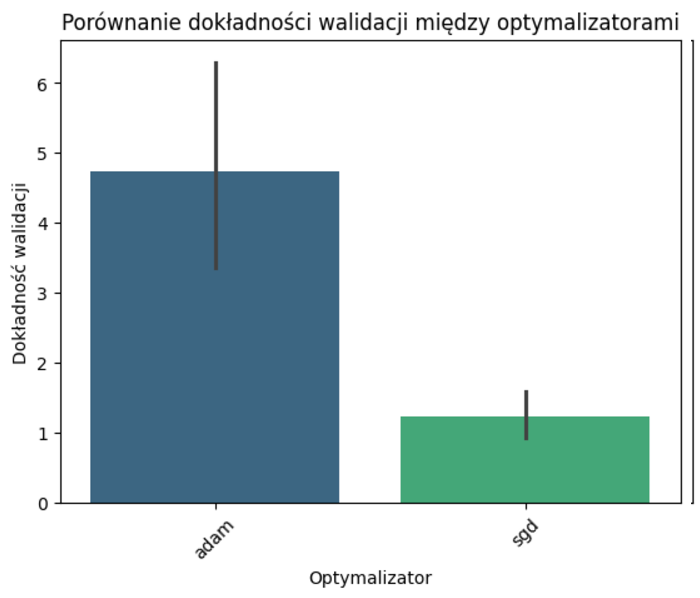
\includegraphics[width=0.6\linewidth]{wal}
	\caption{Czas treningu}
	\label{fig:wal}
\end{figure}
Rysunek 2 typu scatterplot ilustruje zależność między czasem trenowania modelu (na osi X) a jego dokładnością walidacji (na osi Y). Punkty na wykresie reprezentują różne optymalizatory i funkcje aktywacji, a ich rozmieszczenie wskazuje, jak czas treningu wpływa na osiąganą dokładność. Każdy punkt jest oznaczony różnym kolorem w zależności od używanego optymalizatora, co pozwala na rozróżnienie wpływu różnych optymalizatorów na wyniki. Dodatkowo, styl punktów wskazuje, która funkcja aktywacji została zastosowana w modelu, co umożliwia ocenę, jak ta zmienna również wpływa na wydajność modeli. Wykres zawiera legendę, która wskazuje, który kolor odpowiada któremu optymalizatorowi oraz jaką funkcję aktywacji reprezentuje dany styl punktu. Dzięki temu wykresowi można szybko zobaczyć, czy istnieje korelacja między czasem trenowania a dokładnością, a także jak różne optymalizatory i funkcje aktywacji wpływają na efektywność modeli.


%\begin{lstlisting}[language=Python]
%	sns.scatterplot(
%	x='Czas trenowania (s)', 
%	y='Dokladnosc walidacji', 
%	hue='Optymalizator', 
%	style='Funkcja aktywacji', 
%	data=df,
%	palette='deep'
%	)
%	plt.title('Relacja miedzy czasem trenowania a dokladnoscia walidacji')
%	plt.xlabel('Czas trenowania (s)')
%	plt.ylabel('Dokladnosc walidacji')
%	plt.legend(title='Optymalizator i aktywacja')
%	plt.show()
%\end{lstlisting}
\begin{figure}[ht]
	\centering
	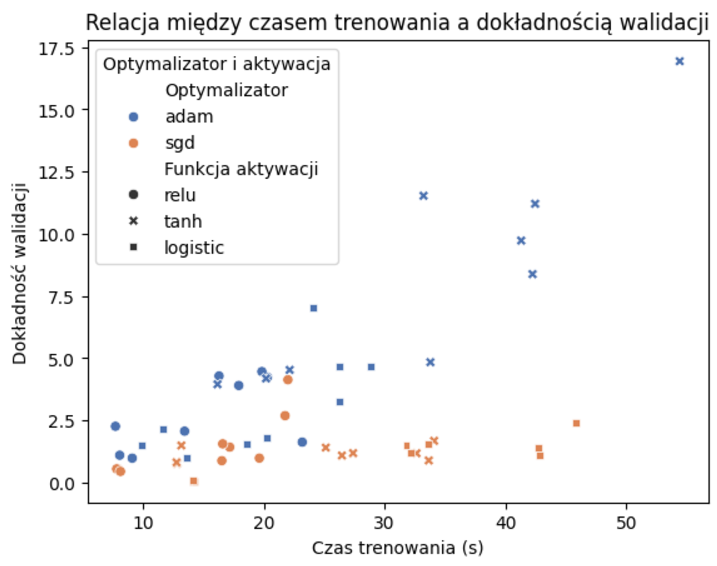
\includegraphics[width=0.6\linewidth]{rela}
	\caption{Czas treningu}
	\label{fig:rela}
\end{figure}

Ostatecznie, porównanie wyników uzyskanych przez różne metody jest przedstawione na Rysunku 4. Zgodnie z wykresem, metoda stacking osiąga średnio lepsze wyniki w porównaniu do baggingu i boosting. Stacking, który polega na łączeniu predykcji różnych klasyfikatorów bazowych przy użyciu modelu drugiego poziomu (meta-learnera), wydaje się skuteczniejszy w wykorzystywaniu różnorodności wyników uzyskanych przez modele bazowe.


\begin{figure}[ht]
	\centering
	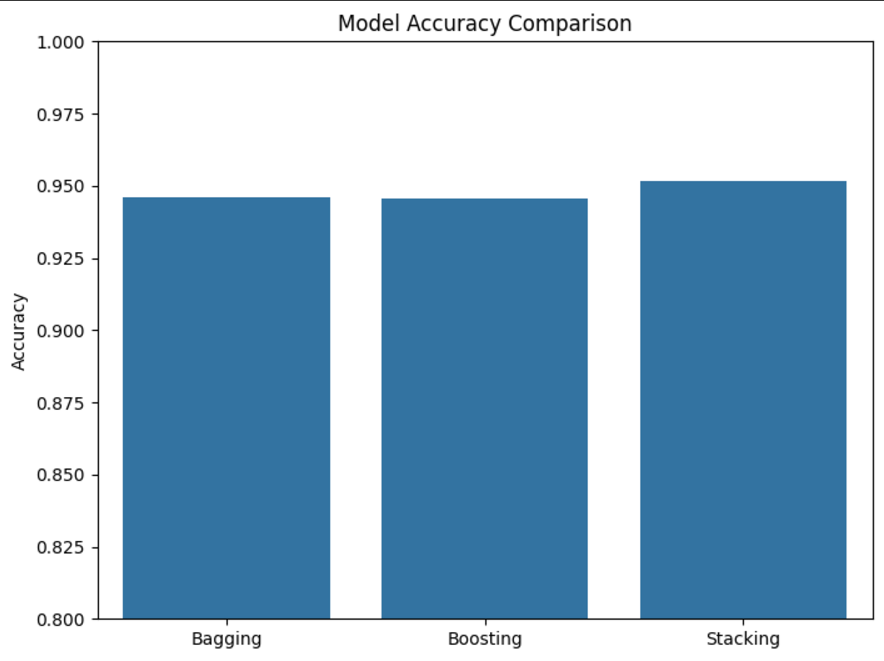
\includegraphics[width=0.6\linewidth]{100accuracy}
	\caption{Czas treningu}
	\label{fig:a}
\end{figure}

\section{Wnioski}
Porównywanie wyników uzyskanych przez różne modele klasyfikacyjne, bazujących na odmiennych założeniach teoretycznych i strukturach wewnętrznych, jest z metodologicznego punktu widzenia nieadekwatne. Brak pełnej znajomości struktury przestrzeni problemowej, w której operują te modele, stanowi kluczowy czynnik uniemożliwiający rzetelną interpretację wyników.



 Niejednorodność struktur wewnętrznych sprawia, że porównanie wyników tych modeli jest nieadekwatne bez uwzględnienia potencjalnych różnic w przestrzeni cech. Przestrzeń problemowa, w której modele te operują, jest często nieliniowa, skomplikowana i zależna od specyfiki zbioru danych. Bez pełnej wiedzy o jej strukturze, nawet dokładne wyniki jednego modelu mogą być nieodpowiednie lub źle zinterpretowane w kontekście innego, co prowadzi do błędnych wniosków.

W związku z tym, brak pełnej świadomości tego, jak dany algorytm przetwarza dane, w jaki sposób interpretuje zależności pomiędzy cechami, a także w jaki sposób przebiega optymalizacja, sprawia, że próby porównań pomiędzy algorytmami mogą prowadzić do mylnych wniosków, które zniekształcają rzeczywisty obraz efektywności modeli w kontekście złożoności problemu.

Jeżeli proces, nawet skomplikowany, można opisać analitycznie, zdecydowanie lepiej jest zastosować podejście analityczne. Każdy z modeli może również różnie reagować na różne dane wejściowe, co nie zostało sprawdzone, dlatego z przeprowadzonych badań nie można wyciągnąć poprawnych wniosków. Przeprowadzenie większej liczby badań na sprawdzenie skuteczności działania modeli, czasowo wykracza poza czas przeznaczony na realizację zajęć. (mam nadzieję, że to nic złego że próbowałem Pythona zamiast Weki, ale ciekawiło mnie jak to by działa :). 

Ogólnie czas uzyskiwania tabelki na końcu to trochę ponad 2 godziny. Ciekawe jest też to, że można było wygenerować dane bezpośrednio do formuły Latex z  poziomu Pythona. Tylko się nie mieściła na stornie, ale można ją przybliżyć w pdf i nie powinna tracić jakości. 


\clearpage

% Wstawienie obróconego pliku PDF
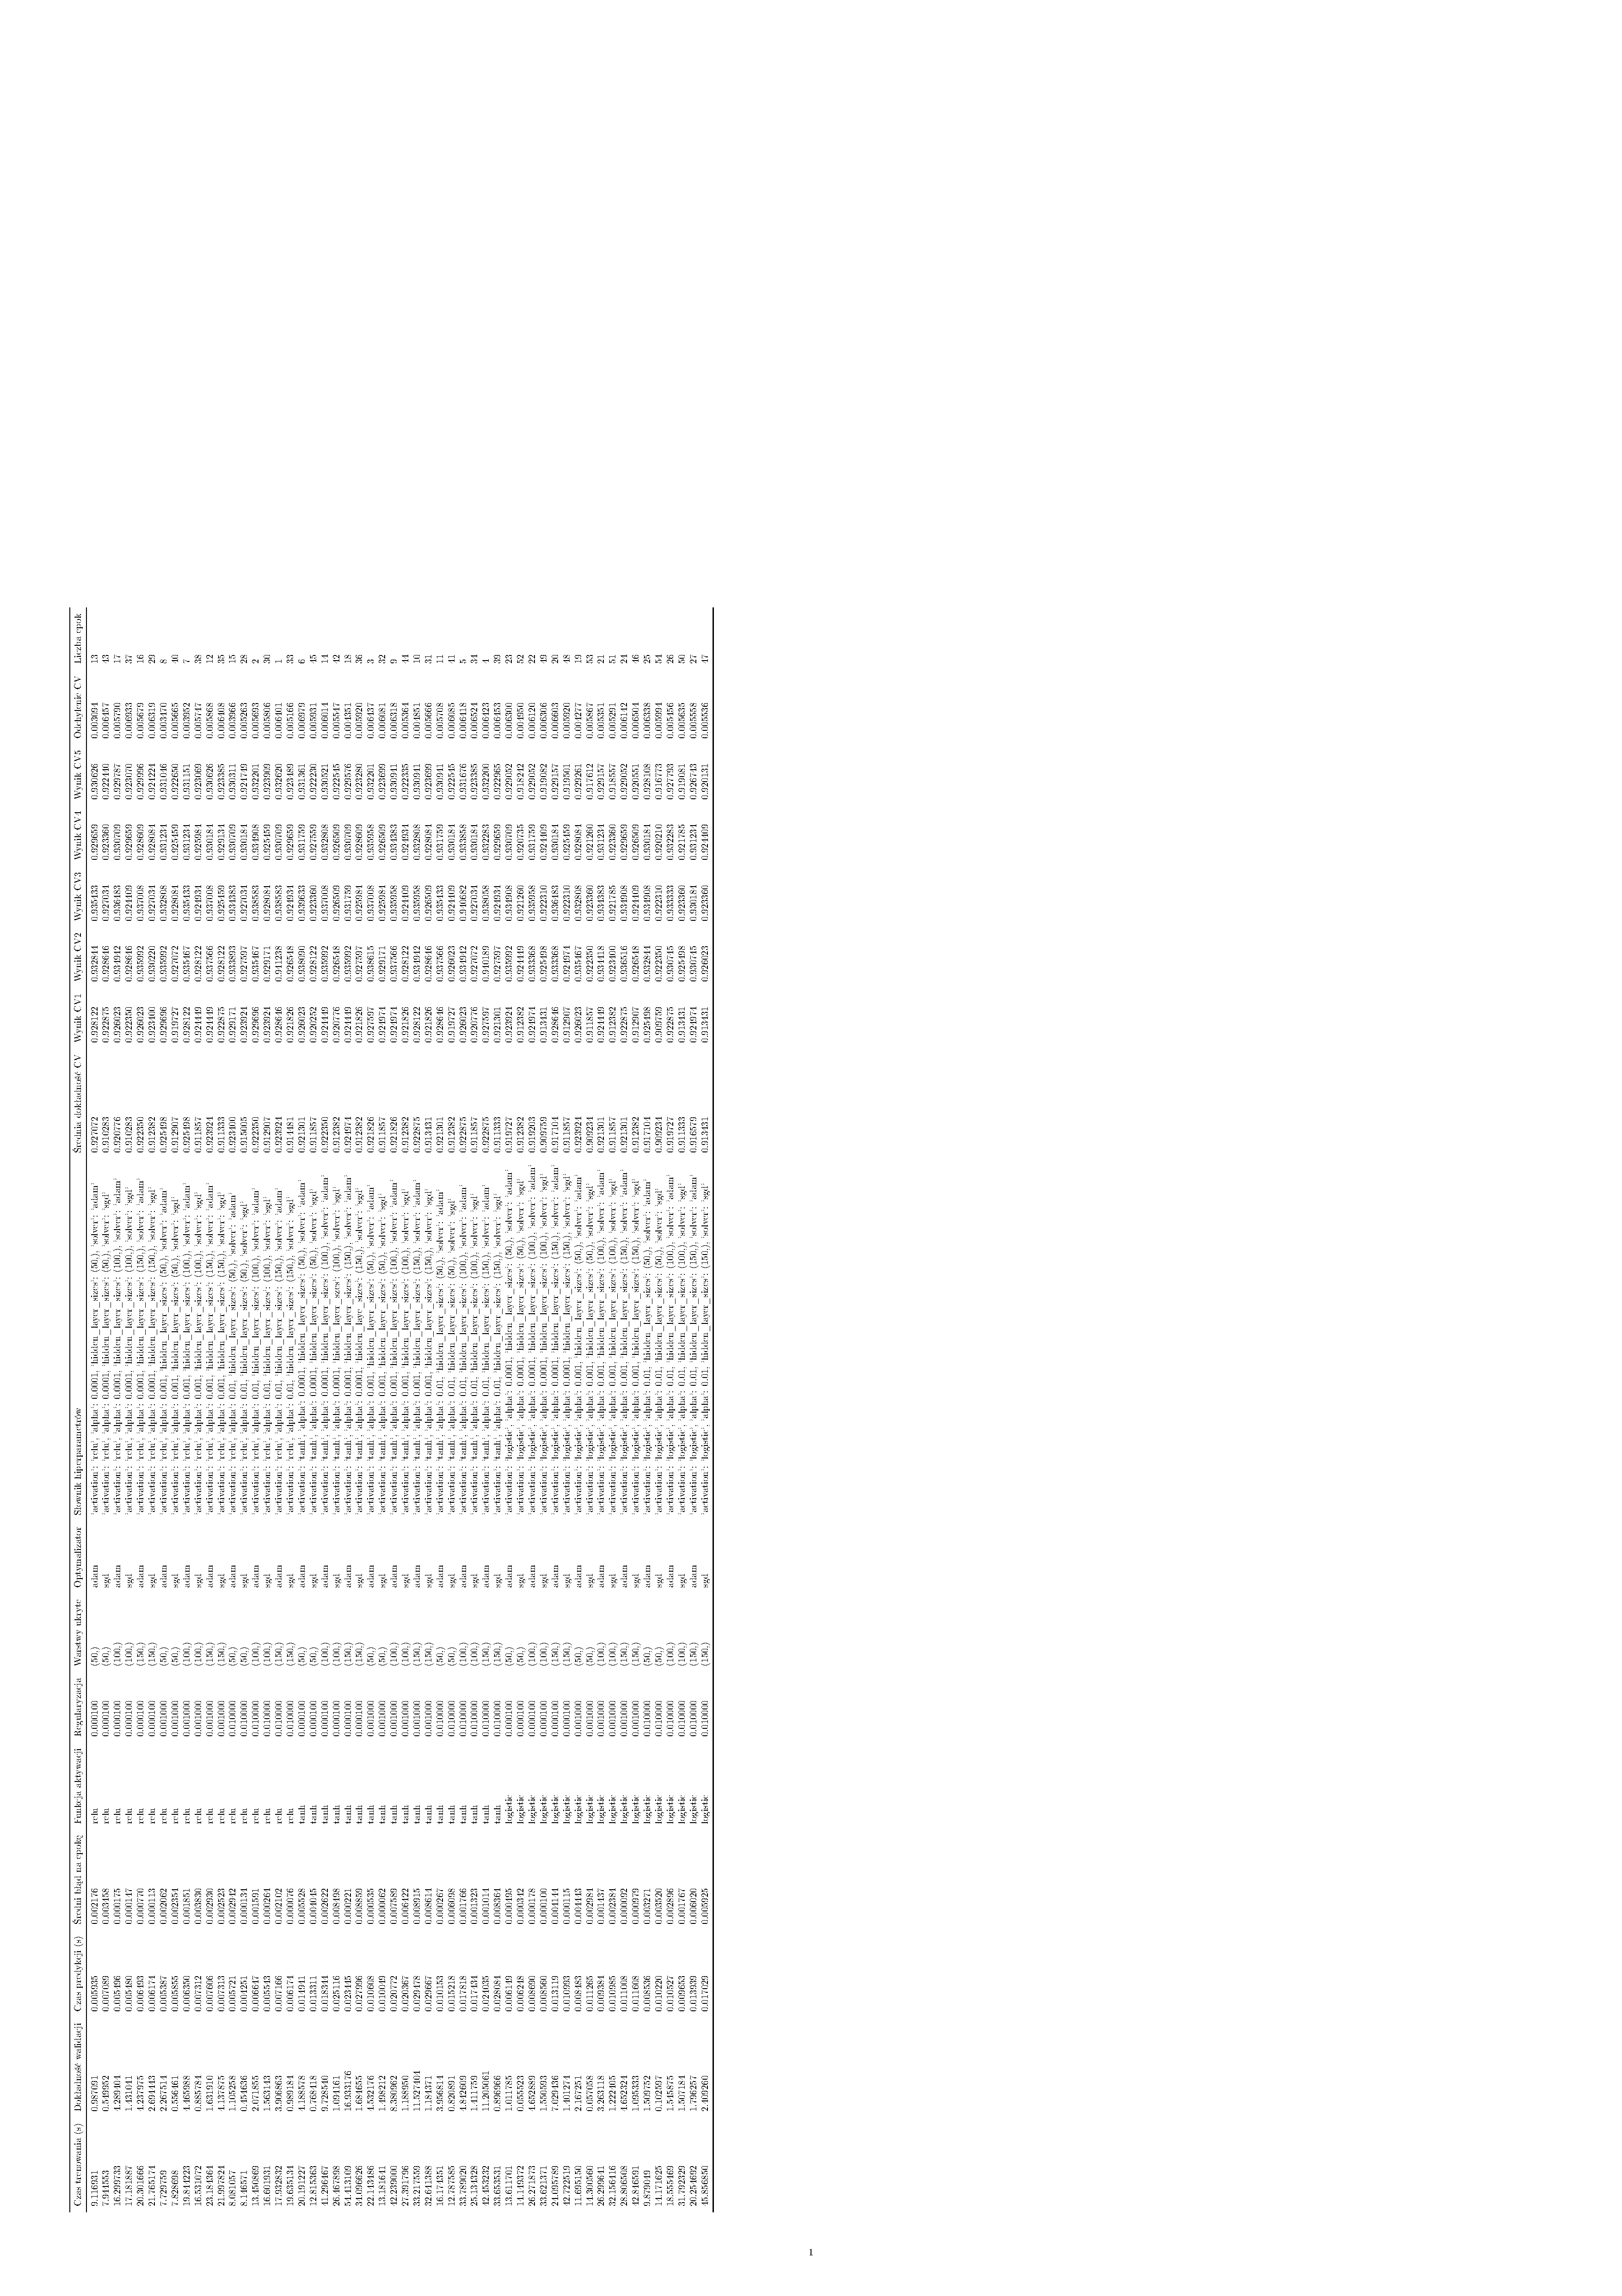
\includepdf[pages=1]{tabela.pdf}
\end{document}
